\documentclass{article}

% content/resources/templates/preamble.tex
\usepackage[margin=0.6in]{geometry}
\author{Milav Dabgar}
\usepackage{amsmath,amssymb,amsthm}
\usepackage{booktabs}
\usepackage{multirow}
\usepackage{xcolor}
\usepackage{tcolorbox}
\tcbuselibrary{breakable,skins}
\usepackage[colorlinks=true,linkcolor=blue]{hyperref}
\usepackage{titlesec}
\usepackage{enumitem}
\usepackage{tikz}
\usepackage{pgfplots}
\usepackage{circuitikz}
\usepackage[version=4]{mhchem}
\usepackage{longtable}
\usepackage{array}
\usepackage{float}
\usepackage{caption}
\usepackage{listings}

\lstset{
  basicstyle=\small\ttfamily,
  breaklines=true,
  breakatwhitespace=false,
  postbreak=\mbox{\textcolor{red}{$\hookrightarrow$}\space},
  float=false,
  numbers=left,
  numberstyle=\tiny\color{gray},
  numbersep=10pt,
  xleftmargin=2em,
  keywordstyle=\color{blue},
  commentstyle=\color{green!60!black},
  stringstyle=\color{purple},
  backgroundcolor=\color{gray!5},
  showstringspaces=false,
  tabsize=2,
  captionpos=b,
  keepspaces=true,
  columns=flexible
}

\pgfplotsset{compat=1.18}
\usetikzlibrary{shapes,arrows,positioning,calc,patterns,decorations.pathmorphing,decorations.markings,arrows.meta}

% Color scheme
\definecolor{headcolor}{RGB}{0,102,204}
\definecolor{keycolor}{RGB}{220,20,60}
\definecolor{solutioncolor}{RGB}{34,139,34}
\definecolor{mnemoniccolor}{RGB}{148,0,211}
\definecolor{codecolor}{RGB}{0,0,100}

% Spacing
\setlength{\parskip}{3pt}
\setlist[itemize]{nosep}
\setlist[enumerate]{nosep}

% Title formatting
\titleformat{\section}{\Large\bfseries\color{headcolor}}{\thesection}{1em}{}
\titleformat{\subsection}{\large\bfseries\color{headcolor}}{\thesubsection}{1em}{}

% Pandoc tightlist compatibility
\providecommand{\tightlist}{%
  \setlength{\itemsep}{0pt}\setlength{\parskip}{0pt}}

% Pandoc longtable compatibility
\newcounter{none}
\def\thenone{}


% content/resources/templates/english-boxes.tex

% Custom environments
\newtcolorbox{solutionbox}{
 breakable,
 enhanced,
 colback=solutioncolor!5!white,
 colframe=solutioncolor!75!black,
 fonttitle=\bfseries,
 title=Solution
}

\newtcolorbox{solutionboxnobreak}{
 colback=solutioncolor!5!white,
 colframe=solutioncolor!75!black,
 fonttitle=\bfseries,
 title=Solution
}

\newtcolorbox{keyformula}{
 breakable,
 enhanced,
 colback=keycolor!5!white,
 colframe=keycolor!75!black,
 fonttitle=\bfseries,
 title=Key Formula
}

\newtcolorbox{mnemonicboxenv}{
 breakable,
 enhanced,
 colback=mnemoniccolor!5!white,
 colframe=mnemoniccolor!75!black,
 fonttitle=\bfseries,
 title=Mnemonic
}

\newcommand{\mnemonicbox}[1]{%
  \begin{mnemonicboxenv}
    #1
  \end{mnemonicboxenv}
}


% Custom commands for GTU solutions
% This file defines semantic commands for consistent formatting

% Question command with automatic formatting
\newcommand{\question}[2]{%
  \section*{Question #1}%
  \textbf{#2}%
}

% OR question variant
\newcommand{\questionor}[2]{%
  \section*{Question #1 OR}%
  \textbf{#2}%
}

% Proper table environment with caption
\newenvironment{answertable}[1]{%
  \begin{table}[htbp]
  \centering
  \caption{#1}
}{%
  \end{table}
}

% Proper figure environment for diagrams
\newenvironment{answerdiagram}[1]{%
  \begin{figure}[htbp]
  \centering
  \caption{#1}
}{%
  \end{figure}
}

% Semantic markup for key terms
\newcommand{\keyword}[1]{\textbf{#1}}
\newcommand{\code}[1]{\texttt{#1}}
\newcommand{\classname}[1]{\texttt{#1}}
\newcommand{\methodname}[1]{\texttt{#1}}

% Proper quotation marks
\newcommand{\mnemonic}[1]{``#1''}


\title{Electronic Circuits \& Applications (4321103) - Winter 2023 Solution}
\date{January 20, 2023}

\begin{document}
\maketitle

\tikzset{
  wave/.style={decorate, decoration={snake, amplitude=.4mm, segment length=2mm, post length=1mm}}
}


\questionmarks{1}{a}{3}
\textbf{What is transistor biasing? What is its need?}

\begin{solutionbox}
\textbf{Answer}:
Transistor biasing is the process of establishing a stable DC operating point (Q-point) for proper amplification of AC signals.

\begin{center}
\captionof{table}{Need for Transistor Biasing}
\begin{tabular}{|l|l|}
\hline
\textbf{Aspect} & \textbf{Importance} \\ \hline
Stability & Maintains stable Q-point despite temperature variations \\ \hline
Linearity & Ensures operation in linear region for distortion-free amplification \\ \hline
Efficiency & Prevents signal clipping and maximizes signal swing \\ \hline
Reliability & Avoids thermal runaway and protects the transistor \\ \hline
\end{tabular}
\end{center}
\end{solutionbox}
\begin{mnemonicbox}
``SOLE operation'' (Stability, Operating point, Linearity, Efficiency)
\end{mnemonicbox}

\questionmarks{1}{b}{4}
\textbf{Explain load line for CE amplifier}

\begin{solutionbox}
\textbf{Answer}:
Load line is a graphical representation of all possible operating points of a transistor circuit.

\begin{center}
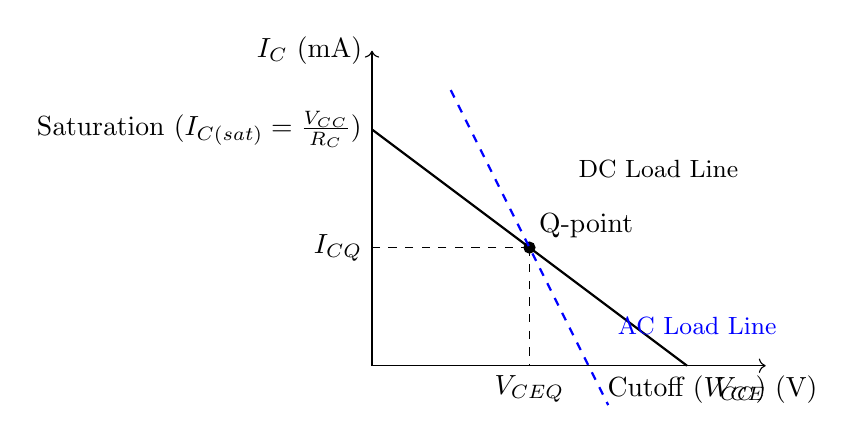
\begin{tikzpicture}[scale=1]
    \draw[<->] (0,4) node[left] {$I_C$ (mA)} -- (0,0) -- (5,0) node[below] {$V_{CE}$ (V)};
    \draw[thick] (0,3) node[left] {Saturation ($I_{C(sat)} = \frac{V_{CC}}{R_C}$)} -- (4,0) node[below] {Cutoff ($V_{CC}$)};
    
    % DC Load Line
    \node [right, align=left] at (2.5, 2.5) {\small DC Load Line};
    
    % Q-Point
    \filldraw (2,1.5) circle (2pt) node[above right] {Q-point};
    \draw[dashed] (2,1.5) -- (2,0) node[below] {$V_{CEQ}$};
    \draw[dashed] (2,1.5) -- (0,1.5) node[left] {$I_{CQ}$};
    
    % AC Load Line - steeper
     \draw[thick, dashed, blue] (1,3.5) -- (3, -0.5);
    \node [right, blue] at (3, 0.5) {\small AC Load Line};

\end{tikzpicture}
\end{center}

\begin{itemize}
    \item \textbf{DC load line}: Drawn between saturation point ($Ic=Vcc/Rc, Vce=0$) and cutoff point ($Ic=0, Vce=Vcc$)
    \item \textbf{AC load line}: Passes through Q-point with slope = $-1/r_c$ ($r_c$ = AC collector resistance)
    \item \textbf{Q-point}: Operating point where DC biasing conditions are established
\end{itemize}
\end{solutionbox}
\begin{mnemonicbox}
``SCQ points'' (Saturation, Cutoff, Q-point)
\end{mnemonicbox}

\questionmarks{1}{c}{7}
\textbf{List various biasing method of transistor and explain any one of them.}

\begin{solutionbox}
\textbf{Answer}:
Various biasing methods for transistors include:

\begin{center}
\captionof{table}{Transistor Biasing Methods}
\begin{tabular}{|l|l|}
\hline
\textbf{Method} & \textbf{Key Feature} \\ \hline
Fixed bias & Single resistor for base bias \\ \hline
Collector-to-base bias & Self-stabilizing due to negative feedback \\ \hline
Voltage divider bias & Most stable due to voltage divider network \\ \hline
Emitter bias & Provides excellent stability with emitter resistor \\ \hline
Combination bias & Uses multiple feedback paths for optimal stability \\ \hline
\end{tabular}
\end{center}

\textbf{Explanation of Voltage Divider Bias:}

\begin{center}
\begin{circuitikz}[scale=0.9, transform shape]
    \draw (0,0) node[npn] (Q) {};
    \draw (Q.C) to[R, l=$R_C$] (0,3) -- (0,4) node[vcc]{$+V_{CC}$};
    \draw (Q.E) to[R, l=$R_E$] (0,-2) node[ground]{};
    
    \draw (Q.B) -- (-1.5,0);
    \draw (-1.5,0) to[R, l=$R_2$] (-1.5,-2) node[ground]{};
    \draw (-1.5,0) to[R, l=$R_1$] (-1.5,4) -- (0,4);
    
    \draw (Q.C) to[short, -o] (1,1) node[right]{Output};
    \draw (Q.C) to[C] (2,1); % Coupling cap at output normally
    
    \draw (-1.5,0) to[C] (-3,0) node[left]{Input};
\end{circuitikz}
\end{center}

\begin{itemize}
    \item \textbf{Operation}: $R_1$ and $R_2$ form a voltage divider to set base voltage
    \item \textbf{Stability}: Excellent thermal stability due to stiff voltage divider
    \item \textbf{Efficiency}: Most widely used due to independence from $\beta$ variations
    \item \textbf{Calculation}: Base voltage = $V_{CC} \times R_2/(R_1+R_2)$
\end{itemize}
\end{solutionbox}
\begin{mnemonicbox}
``VISE grip'' (Voltage divider, Independent of $\beta$, Stable, Efficient)
\end{mnemonicbox}

\orquestionmarks{1}{c}{7}
\textbf{Explain voltage divider biasing method with help of circuit diagram}

\begin{solutionbox}
\textbf{Answer}:
Voltage divider biasing is the most stable method to bias a transistor.

\begin{center}
\begin{circuitikz}[scale=0.9, transform shape]
    \draw (0,0) node[npn] (Q) {};
    \draw (Q.C) to[R, l=$R_C$] (0,3) -- (0,4) node[vcc]{$+V_{CC}$};
    \draw (Q.E) to[R, l=$R_E$] (0,-2) node[ground]{};
    \draw (Q.E) -- (1,-2) to[C, l=$C_E$] (1,-4) node[ground]{}; % Bypass cap often included in full diagrams
    
    \draw (Q.B) -- (-1.5,0);
    \draw (-1.5,0) to[R, l=$R_2$] (-1.5,-2) node[ground]{};
    \draw (-1.5,0) to[R, l=$R_1$] (-1.5,4) -- (0,4);
    
    \draw (Q.C) to[C, l=$C_C$] (2,1.5) node[right]{Output};
    \draw (-1.5,0) to[C, l=$C_C$] (-3,0) node[left]{Input};
\end{circuitikz}
\end{center}

\begin{center}
\captionof{table}{Features of Voltage Divider Biasing}
\begin{tabular}{|l|l|}
\hline
\textbf{Component} & \textbf{Function} \\ \hline
$R_1, R_2$ & Creates stable base voltage independent of $\beta$ \\ \hline
$R_C$ & Limits collector current and develops output voltage \\ \hline
$R_E$ & Provides stability via negative feedback \\ \hline
Bypass capacitor & Bypasses AC signal around $R_E$ to increase gain \\ \hline
\end{tabular}
\end{center}

\begin{itemize}
    \item \textbf{Working principle}: $R_1$ and $R_2$ form a voltage divider that sets the base voltage
    \item \textbf{Thermal stability}: $R_E$ provides negative feedback for excellent thermal stability
    \item \textbf{Advantage}: Q-point remains stable despite variations in temperature and $\beta$
\end{itemize}
\end{solutionbox}
\begin{mnemonicbox}
``BEST bias'' (Base voltage, Emitter stability, Stiff divider, Temperature stable)
\end{mnemonicbox}

\questionmarks{2}{a}{3}
\textbf{Write methods of cascading amplifiers}

\begin{solutionbox}
\textbf{Answer}:
Cascading amplifiers means connecting multiple amplifier stages in series to increase overall gain.

\begin{center}
\captionof{table}{Methods of Cascading Amplifiers}
\begin{tabular}{|l|l|}
\hline
\textbf{Method} & \textbf{Key Feature} \\ \hline
RC Coupling & Uses capacitor and resistor for interstage coupling \\ \hline
Transformer Coupling & Uses transformer for impedance matching and isolation \\ \hline
Direct Coupling & No coupling components, direct connection between stages \\ \hline
LC Coupling & Uses inductor-capacitor for high-frequency applications \\ \hline
\end{tabular}
\end{center}
\end{solutionbox}
\begin{mnemonicbox}
``RTDL connection'' (RC, Transformer, Direct, LC)
\end{mnemonicbox}

\questionmarks{2}{b}{4}
\textbf{Compare CE and CB amplifiers}

\begin{solutionbox}
\textbf{Answer}:

\begin{center}
\captionof{table}{Comparison of CE and CB Amplifiers}
\begin{tabular}{|l|l|l|}
\hline
\textbf{Parameter} & \textbf{Common Emitter (CE)} & \textbf{Common Base (CB)} \\ \hline
Input Impedance & Medium ($\approx$1k$\Omega$) & Low ($\approx$50$\Omega$) \\ \hline
Output Impedance & High ($\approx$50k$\Omega$) & Very high ($\approx$500k$\Omega$) \\ \hline
Voltage Gain & High ($\approx$500) & High ($\approx$500) \\ \hline
Current Gain & Medium ($\beta$) & Less than 1 ($\alpha$) \\ \hline
Phase Shift & 180$^{\circ}$ & 0$^{\circ}$ \\ \hline
Applications & Voltage amplification & High-frequency amplification \\ \hline
\end{tabular}
\end{center}
\end{solutionbox}
\begin{mnemonicbox}
``PIVOT differences'' (Phase shift, Impedance, Voltage gain, Output impedance, Throughput)
\end{mnemonicbox}

\questionmarks{2}{c}{7}
\textbf{Draw the circuit of RC coupled amplifier. Give the frequency response and explain}

\begin{solutionbox}
\textbf{Answer}:
RC coupled amplifier uses resistor-capacitor network for interstage coupling.

\begin{center}
\begin{circuitikz}[scale=0.8, transform shape]
    % Stage 1
    \draw (0,0) node[npn] (Q1) {Q1};
    \draw (Q1.E) to[R, l=$R_{E1}$] (0,-2) node[ground]{};
    \draw (Q1.C) to[R, l=$R_{C1}$] (0,2) -- (0,3) node[vcc]{$+V_{CC}$};
    \draw (Q1.B) to[R, l=$R_{2}$] (-1,-2) node[ground]{};
    \draw (Q1.B) to[R, l=$R_{1}$] (-1,2) -- (0,2);
    \draw (Q1.B) to[C, l=$C_{in}$] (-2.5,0) node[left]{Input};
    
    % Coupling
    \draw (Q1.C) to[C, l=$C_C$] (2,0.5) -- (3,0); % To base of Q2
    
    % Stage 2
    \draw (4,0) node[npn] (Q2) {Q2};
    \draw (Q2.E) to[R, l=$R_{E2}$] (4,-2) node[ground]{};
    \draw (Q2.C) to[R, l=$R_{C2}$] (4,2) -- (4,3) -- (0,3);
    \draw (3,0) -- (Q2.B);
    \draw (3,0) to[R, l=$R'_{2}$] (3,-2) node[ground]{};
    \draw (3,0) to[R, l=$R'_{1}$] (3,2) -- (4,2);
    
    \draw (Q2.C) to[C, l=$C_{out}$] (6,1) node[right]{Output};
\end{circuitikz}
\end{center}

\textbf{Frequency Response:}

\begin{center}
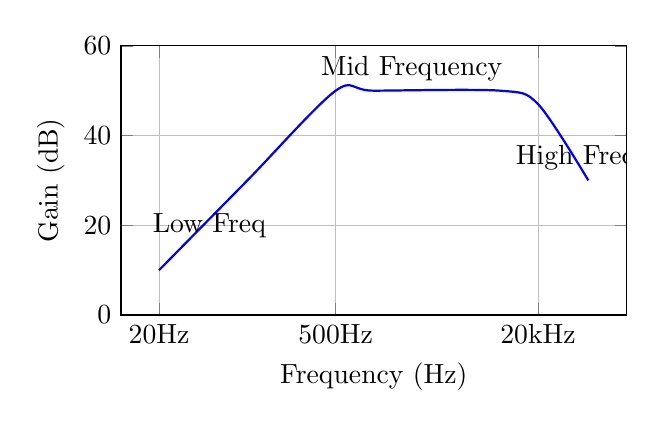
\begin{tikzpicture}
    \begin{semilogxaxis}[
        width=8cm, height=5cm,
        xlabel={Frequency (Hz)},
        ylabel={Gain (dB)},
        xmin=10, xmax=100000,
        ymin=0, ymax=60,
        xtick={20, 500, 20000},
        xticklabels={20Hz, 500Hz, 20kHz},
        grid=major
    ]
    \addplot[thick, smooth, blue] coordinates {
        (20, 10) (100, 30) (500, 50) (1000, 50) (10000, 50) (20000, 47) (50000, 30)
    };
    \node at (axis cs: 50, 20) {Low Freq};
    \node at (axis cs: 2000, 55) {Mid Frequency};
    \node at (axis cs: 40000, 35) {High Freq};
    \end{semilogxaxis}
\end{tikzpicture}
\end{center}

\begin{itemize}
    \item \textbf{Low frequency region}: Gain drops due to coupling and bypass capacitors
    \item \textbf{Mid frequency region}: Flat response with maximum gain
    \item \textbf{High frequency region}: Gain falls due to transistor internal capacitances
    \item \textbf{Bandwidth}: Determined by the lower and upper cutoff frequencies
\end{itemize}
\end{solutionbox}
\begin{mnemonicbox}
``LMH regions'' (Low, Mid, High frequency regions)
\end{mnemonicbox}

\orquestionmarks{2}{a}{3}
\textbf{Write definition of gain, Bandwidth and Gain Bandwidth product of an amplifier.}

\begin{solutionbox}
\textbf{Answer}:

\begin{center}
\captionof{table}{Key Amplifier Parameters}
\begin{tabular}{|l|p{8cm}|}
\hline
\textbf{Parameter} & \textbf{Definition} \\ \hline
Gain (A) & Ratio of output signal to input signal (voltage, current, or power) \\ \hline
Bandwidth (BW) & Frequency range between lower and upper cutoff frequencies ($f_2-f_1$) \\ \hline
Gain-Bandwidth Product (GBW) & Product of gain and bandwidth, remains constant for a given amplifier \\ \hline
\end{tabular}
\end{center}
\end{solutionbox}
\begin{mnemonicbox}
``GBP constants'' (Gain, Bandwidth, Product constants)
\end{mnemonicbox}

\orquestionmarks{2}{b}{4}
\textbf{Explain frequency response of single stage amplifier and indicate its cutoff frequencies.}

\begin{solutionbox}
\textbf{Answer}:
Frequency response shows variation of gain with frequency in a single stage amplifier.

\begin{center}
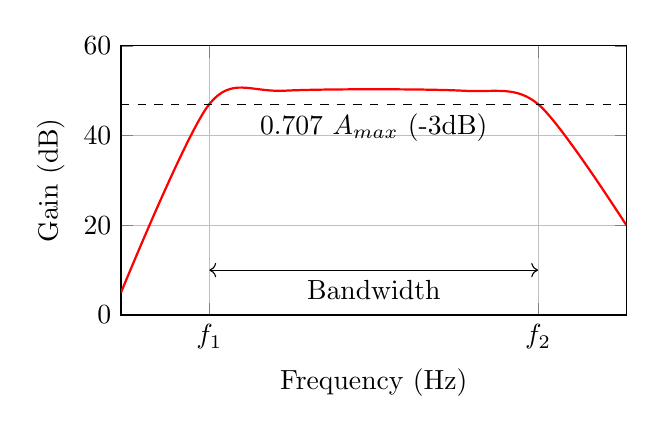
\begin{tikzpicture}
    \begin{semilogxaxis}[
        width=8cm, height=5cm,
        xlabel={Frequency (Hz)},
        ylabel={Gain (dB)},
        xmin=10, xmax=100000,
        ymin=0, ymax=60,
        xtick={50, 20000},
        xticklabels={$f_1$, $f_2$},
        grid=major
    ]
    \addplot[thick, smooth, red] coordinates {
        (10, 5) (50, 47) (200, 50) (5000, 50) (20000, 47) (100000, 20)
    };
    \draw[dashed, black] (axis cs: 10, 47) -- (axis cs: 100000, 47) node[midway, below] {0.707 $A_{max}$ (-3dB)};
    \draw[<->] (axis cs: 50, 10) -- (axis cs: 20000, 10) node[midway, below] {Bandwidth};
    \end{semilogxaxis}
\end{tikzpicture}
\end{center}

\begin{itemize}
    \item \textbf{Cutoff frequencies}: Points where gain drops to 0.707 times maximum gain
    \item \textbf{Lower cutoff frequency ($f_1$)}: Determined by coupling and bypass capacitors
    \item \textbf{Upper cutoff frequency ($f_2$)}: Limited by transistor junction capacitances
    \item \textbf{Bandwidth}: Frequency range between $f_1$ and $f_2$ ($BW = f_2 - f_1$)
\end{itemize}
\end{solutionbox}
\begin{mnemonicbox}
``LUG points'' (Lower cutoff, Upper cutoff, Gain maximum)
\end{mnemonicbox}

\orquestionmarks{2}{c}{7}
\textbf{Draw and Explain circuit diagram of common collector amplifier}

\begin{solutionbox}
\textbf{Answer}:
Common collector (CC) amplifier is also known as emitter follower.

\begin{center}
\begin{circuitikz}[scale=0.9, transform shape]
    \draw (0,0) node[npn] (Q) {};
    \draw (Q.C) -- (0,2) node[vcc]{$+V_{CC}$}; % Collector to Vcc directly or via resistor? Usually direct for CC
    \draw (Q.E) to[R, l=$R_E$] (0,-2) node[ground]{};
    
    \draw (Q.B) to[C, l=$C_{in}$] (-2,0) node[left]{Input};
    \draw (Q.B) to[R, l=$R_B$] (-0.5,-2) node[ground]{}; % Simplified biasing
    
    \draw (Q.E) to[C, l=$C_{out}$] (2,-0.5) node[right]{Output};
\end{circuitikz}
\end{center}

\begin{center}
\captionof{table}{Features of Common Collector Amplifier}
\begin{tabular}{|l|l|}
\hline
\textbf{Parameter} & \textbf{Characteristic} \\ \hline
Voltage Gain & Approximately 1 (less than 1) \\ \hline
Current Gain & High ($\beta$) \\ \hline
Input Impedance & Very high ($\approx \beta \times R_E$) \\ \hline
Output Impedance & Very low ($\approx 1/g_m$) \\ \hline
Phase Shift & 0$^{\circ}$ (no phase inversion) \\ \hline
Applications & Impedance matching, buffer stages \\ \hline
\end{tabular}
\end{center}

\begin{itemize}
    \item \textbf{Working principle}: Output is taken from emitter, collector is common to input and output
    \item \textbf{Key feature}: Voltage follower with output voltage following input voltage
    \item \textbf{Main advantage}: High input impedance and low output impedance
\end{itemize}
\end{solutionbox}
\begin{mnemonicbox}
``BIVOP characters'' (Buffer, Impedance matching, Voltage follower, One gain, Phase matched)
\end{mnemonicbox}

\questionmarks{3}{a}{3}
\textbf{Draw transistor two port network and describe h-parameters for it.}

\begin{solutionbox}
\textbf{Answer}:
Transistor can be represented as a two-port network with h-parameters.

\begin{center}
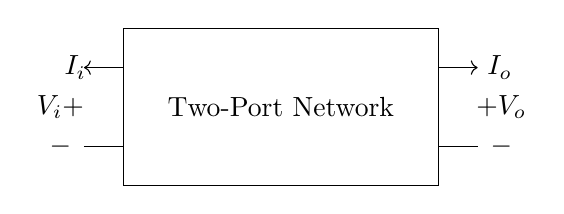
\begin{tikzpicture}[node distance=2cm, auto]
    \draw (0,0) rectangle (4,2);
    \node at (2,1) {Two-Port Network};
    
    % Input Port
    \draw [<-] (-0.5, 1.5) -- (0, 1.5) node[left, xshift=-10pt] {$I_i$};
    \draw (-0.5, 0.5) -- (0, 0.5);
    \node at (-0.8, 1) {$V_i +$};
    \node at (-0.8, 0.5) {$ - $};
    
    % Output Port
    \draw [->] (4, 1.5) -- (4.5, 1.5) node[right] {$I_o$};
    \draw (4, 0.5) -- (4.5, 0.5);
    \node at (4.8, 1) {$+ V_o$};
    \node at (4.8, 0.5) {$ - $};
\end{tikzpicture}
\end{center}

\begin{center}
\captionof{table}{h-parameters}
\begin{tabular}{|l|l|}
\hline
\textbf{Parameter} & \textbf{Description} \\ \hline
$h_{11} (h_i)$ & Input impedance with output short-circuited \\ \hline
$h_{12} (h_r)$ & Reverse voltage transfer ratio with input open-circuited \\ \hline
$h_{21} (h_f)$ & Forward current transfer ratio with output short-circuited \\ \hline
$h_{22} (h_o)$ & Output admittance with input open-circuited \\ \hline
\end{tabular}
\end{center}
\end{solutionbox}
\begin{mnemonicbox}
``IRFO parameters'' (Input impedance, Reverse transfer, Forward transfer, Output admittance)
\end{mnemonicbox}

\questionmarks{3}{b}{4}
\textbf{Explain voltage gain Av, current gain Ai and Power gain Ap for CE amplifier}

\begin{solutionbox}
\textbf{Answer}:

\begin{center}
\captionof{table}{Gain Expressions for CE Amplifier}
\begin{tabular}{|l|l|p{4cm}|}
\hline
\textbf{Gain Type} & \textbf{Expression} & \textbf{Relation to h-parameters} \\ \hline
Voltage Gain ($A_v$) & $V_o/V_i$ & $A_v = -h_{fe} \times R_L / h_{ie}$ \\ \hline
Current Gain ($A_i$) & $I_o/I_i$ & $A_i = h_{fe} / (1 + h_{oe} \times R_L)$ \\ \hline
Power Gain ($A_p$) & $P_o/P_i$ & $A_p = A_v \times A_i$ \\ \hline
\end{tabular}
\end{center}

\begin{itemize}
    \item \textbf{Voltage gain}: Typically 500-1000 for CE amplifier
    \item \textbf{Current gain}: Approximately equal to $h_{fe}$ ($\beta$) of transistor
    \item \textbf{Power gain}: Product of voltage gain and current gain
\end{itemize}
\end{solutionbox}
\begin{mnemonicbox}
``VIP gains'' (Voltage, Input-output current, Power)
\end{mnemonicbox}

\questionmarks{3}{c}{7}
\textbf{Explain Darlington pair, its features and applications}

\begin{solutionbox}
\textbf{Answer}:
Darlington pair consists of two transistors connected to act as a single high-gain transistor.

\begin{center}
\begin{circuitikz}
    \draw (0,0) node[npn] (Q1) {Q1};
    \draw (2,0) node[npn] (Q2) {Q2};
    \draw (Q1.C) -- (Q2.C) -- ++(0,0.5) node[vcc]{C};
    \draw (Q1.E) -- (Q2.B);
    \draw (Q1.B) -- ++(-0.5,0) node[left]{B};
    \draw (Q2.E) -- ++(0,-0.5) node[below]{E};
\end{circuitikz}
\end{center}

\begin{center}
\captionof{table}{Features of Darlington Pair}
\begin{tabular}{|l|l|}
\hline
\textbf{Feature} & \textbf{Description} \\ \hline
Current Gain & Very high ($\beta_1 \times \beta_2$) \\ \hline
Input Impedance & Extremely high \\ \hline
Voltage Drop & Higher ($\approx$1.4V) due to two B-E junctions \\ \hline
Switching Speed & Slower than single transistor \\ \hline
Thermal Stability & Poorer than single transistor \\ \hline
\end{tabular}
\end{center}

\begin{itemize}
    \item \textbf{Applications}: Power amplifiers, motor drivers, touch switches, sensors
    \item \textbf{Advantages}: Very high current gain, high input impedance
    \item \textbf{Limitations}: Higher saturation voltage, slower switching
\end{itemize}
\end{solutionbox}
\begin{mnemonicbox}
``CHIPS application'' (Current amplification, High impedance, Increased gain, Power handling, Slower switching)
\end{mnemonicbox}

\orquestionmarks{3}{a}{3}
\textbf{Discuss applications of LDR.}

\begin{solutionbox}
\textbf{Answer}:
Light Dependent Resistor (LDR) is a photoresistor whose resistance decreases with increasing light intensity.

\begin{center}
\captionof{table}{Applications of LDR}
\begin{tabular}{|l|p{8cm}|}
\hline
\textbf{Application} & \textbf{Working Principle} \\ \hline
Automatic Street Lights & Turns on lights when ambient light level falls \\ \hline
Camera Exposure Control & Adjusts aperture/shutter based on light intensity \\ \hline
Light Beam Alarms & Triggers alarm when light beam is interrupted \\ \hline
Solar Trackers & Helps orient solar panels toward maximum sunlight \\ \hline
Automatic Brightness Control & Adjusts display brightness based on ambient light \\ \hline
\end{tabular}
\end{center}
\end{solutionbox}
\begin{mnemonicbox}
``CASAL applications'' (Camera, Alarm, Street light, Automatic control, Light measurement)
\end{mnemonicbox}

\orquestionmarks{3}{b}{4}
\textbf{Comparison of clipper and clamper}

\begin{solutionbox}
\textbf{Answer}:

\begin{center}
\captionof{table}{Comparison between Clipper and Clamper}
\begin{tabular}{|l|p{4.5cm}|p{4.5cm}|}
\hline
\textbf{Parameter} & \textbf{Clipper} & \textbf{Clamper} \\ \hline
Function & Limits/clips signal amplitude & Shifts DC level of signal \\ \hline
Output & Removes portions beyond threshold & Adds DC component \\ \hline
Components & Diode + Resistor & Diode + Capacitor + Resistor \\ \hline
Wave Shape & Changes wave shape & Preserves wave shape \\ \hline
Applications & Noise removal, wave shaping & TV signal processing, DC restoration \\ \hline
\end{tabular}
\end{center}

\begin{center}
\begin{tikzpicture}[node distance=2cm, auto]
    \node [gtu block] (in) {Input Signal};
    \node [gtu block, right of=in, node distance=3cm] (clip) {Clipper};
    \node [gtu block, below of=clip] (clamp) {Clamper};
    \node [gtu block, right of=clip, node distance=3.5cm] (out_clip) {Ampl. Limited};
    \node [gtu block, right of=clamp, node distance=3.5cm] (out_clamp) {DC Level Shifted};
    
    \draw [gtu arrow] (in) -- (clip);
    \draw [gtu arrow] (in) |- (clamp);
    \draw [gtu arrow] (clip) -- (out_clip);
    \draw [gtu arrow] (clamp) -- (out_clamp);
\end{tikzpicture}
\end{center}
\end{solutionbox}
\begin{mnemonicbox}
``CLIPS vs CLAMPS'' (Cut Levels In Peak Signal vs Change Level And Maintain Peak Shape)
\end{mnemonicbox}

\orquestionmarks{3}{c}{7}
\textbf{Describe h-parameters circuit for CE amplifier.}

\begin{solutionbox}
\textbf{Answer}:
h-parameters provide a simple way to analyze CE amplifier performance.

\begin{center}
\begin{circuitikz}[scale=1]
    \draw (0,0) node[left]{Input} to[short, o-] (1,0) to[R, l=$h_{ie}$] (3,0) to[cV, l=$h_{re}V_{ce}$] (3,-2) to[short, -o] (0,-2) node[left]{Common};
    
    \draw (5,0) to[cI, l=$h_{fe}I_b$, invert] (5,-2);
    \draw (7,0) to[R, l=$\frac{1}{h_{oe}}$] (7,-2); 
    \draw (5,0) to[short, -o] (8,0) node[right]{Output};
    \draw (5,-2) to[short, -o] (8,-2) node[right]{Common};
    
    \node at (0.5, -1) {$V_i$};
    \node at (7.5, -1) {$V_o$};
    \draw[->] (0.2, 0) -- (0.8, 0) node[midway, above] {$I_i$};
    \draw[->] (7.8, 0) -- (7.2, 0) node[midway, above] {$I_o$};
\end{circuitikz}
\end{center}

\begin{center}
\captionof{table}{h-parameters for CE Configuration}
\begin{tabular}{|l|l|l|l|}
\hline
\textbf{Parameter} & \textbf{Symbol} & \textbf{Value} & \textbf{Physical Significance} \\ \hline
Input impedance & $h_{ie}$ & 1-2 k$\Omega$ & Base-emitter input impedance \\ \hline
Reverse ratio & $h_{re}$ & $10^{-4}$ & Feedback from output to input \\ \hline
Forward current gain & $h_{fe}$ & 50-300 & Current gain ($\beta$) \\ \hline
Output admittance & $h_{oe}$ & $10^{-6}$ S & Output conductance \\ \hline
\end{tabular}
\end{center}

\begin{itemize}
    \item \textbf{Circuit analysis}: Uses h-parameters to calculate voltage gain, current gain, input/output impedance
    \item \textbf{Equivalent circuit}: Combines h-parameters in a two-port network representation
    \item \textbf{Advantage}: Simplifies complex transistor behavior into linear parameters
\end{itemize}
\end{solutionbox}
\begin{mnemonicbox}
``FIRO parameters'' (Forward gain, Input impedance, Reverse feedback, Output admittance)
\end{mnemonicbox}

\questionmarks{4}{a}{3}
\textbf{Write short note on Darlington pair.}

\begin{solutionbox}
\textbf{Answer}:
Darlington pair combines two transistors to create a super-high gain transistor.

\begin{center}
\begin{circuitikz}
    \draw (0,0) node[npn] (Q1) {Q1};
    \draw (2,0) node[npn] (Q2) {Q2};
    \draw (Q1.C) -- (Q2.C) -- ++(0,0.5) node[right]{Collector};
    \draw (Q1.E) -- (Q2.B);
    \draw (Q1.B) -- ++(-0.5,0) node[left]{Base};
    \draw (Q2.E) -- ++(0,-0.5) node[below]{Emitter};
\end{circuitikz}
\end{center}

\begin{itemize}
    \item \textbf{Configuration}: Two transistors where first transistor's emitter drives second transistor's base
    \item \textbf{Total gain}: $\beta_1 \times \beta_2$ (product of individual transistor gains)
    \item \textbf{Input impedance}: Extremely high ($\beta_2 \times R_{e1}$)
\end{itemize}
\end{solutionbox}
\begin{mnemonicbox}
``HIS properties'' (High gain, Impedance boost, Sandwich configuration)
\end{mnemonicbox}

\questionmarks{4}{b}{4}
\textbf{Explain Zener diode as a voltage regulator.}

\begin{solutionbox}
\textbf{Answer}:
Zener diode provides a constant voltage reference when operated in reverse breakdown.

\begin{center}
\begin{circuitikz}
    \draw (0,0) to[V, l=$V_{in}$] (0,3) to[R, l=$R_S$] (3,3) -- (5,3) to[R, l=$R_L$] (5,0) -- (0,0);
    \draw (3,3) to[zD, l=$D_Z$, invert] (3,0) node[ground]{};
    \draw (5,3) to[short, -o] (6,3) node[right]{$V_{out}$};
    \draw (5,0) to[short, -o] (6,0);
\end{circuitikz}
\end{center}

\begin{center}
\captionof{table}{Zener Voltage Regulator}
\begin{tabular}{|l|l|}
\hline
\textbf{Parameter} & \textbf{Description} \\ \hline
Principle & Maintains constant voltage in reverse breakdown region \\ \hline
Series Resistor ($R_S$) & Limits current and drops excess voltage \\ \hline
Load Resistor ($R_L$) & Represents the circuit being powered \\ \hline
Regulation & Maintains constant output despite input voltage fluctuations \\ \hline
\end{tabular}
\end{center}

\begin{itemize}
    \item \textbf{Working}: Zener operates in breakdown region, maintaining fixed voltage
    \item \textbf{Limitation}: Power dissipation capability limits maximum current
\end{itemize}
\end{solutionbox}
\begin{mnemonicbox}
``ZEBRA'' (Zener Effect Breakdown Regulates Accurately)
\end{mnemonicbox}

\questionmarks{4}{c}{7}
\textbf{Explain Optocoupler with advantages and disadvantages.}

\begin{solutionbox}
\textbf{Answer}:
Optocoupler (also called optoisolator) uses light to transfer signals between isolated circuits.

\begin{center}
\begin{circuitikz}
    % Input side
    \draw (0,0) node[left]{Input} to[led, l={LED}, photo] (0,-2) node[ground]{};
    \draw (0,0) to[R] (0,2);
    
    % Enclosure
    \draw[dashed, thick] (-1,1) rectangle (3,-1.5);
    \node at (1, -1) {Optocoupler IC};
    
    % Output side
    \draw (2,0) node[npn, photo] (Q) {};
    \draw (Q.C) to[R] (2,2) node[vcc]{$+V_{CC}$};
    \draw (Q.E) node[ground]{};
    \draw (Q.C) to[short, -o] (3,1) node[right]{Output};
    
    % Light waves
    \draw[->, wave] (0.5, -0.5) -- (1.5, -0.5);
    \draw[->, wave] (0.5, -0.8) -- (1.5, -0.8);
\end{circuitikz}
\end{center}

\begin{center}
\captionof{table}{Advantages and Disadvantages of Optocoupler}
\begin{tabular}{|l|l|}
\hline
\textbf{Advantages} & \textbf{Disadvantages} \\ \hline
Complete electrical isolation & Relatively slow response time \\ \hline
High noise immunity & Limited bandwidth \\ \hline
No ground loops & Temperature sensitive \\ \hline
High voltage isolation & Aging effects \\ \hline
Protection against transients & Requires current to drive LED \\ \hline
\end{tabular}
\end{center}

\begin{itemize}
    \item \textbf{Working}: Input signal drives LED, which emits light detected by photodetector
    \item \textbf{Applications}: Medical equipment, industrial control, power supplies, signal isolation
    \item \textbf{Types}: Photoresistor, photodiode, phototransistor, photo-SCR based
\end{itemize}
\end{solutionbox}
\begin{mnemonicbox}
``LIGHT transfer'' (Linked Isolated Galvanic-free High-voltage Transfer)
\end{mnemonicbox}

\orquestionmarks{4}{a}{3}
\textbf{Draw Half Wave Voltage Doubler.}

\begin{solutionbox}
\textbf{Answer}:
Half-wave voltage doubler uses diodes and capacitors to produce DC output approximately twice the peak input voltage.

\begin{center}
\begin{circuitikz}[scale=0.9]
    \draw (0,0) to[sinusoidal voltage source, l=$V_{in}$] (0,2) to[C, l=$C_1$] (2,2);
    \draw (2,2) to[D, l=$D_1$] (2,0) -- (0,0);
    \draw (2,2) to[D, l=$D_2$] (4,2) to[C, l=$C_2$] (4,0) -- (2,0);
    \draw (4,2) to[short, -o] (5,2) node[right]{$V_{out} \approx 2V_m$};
    \draw (4,0) to[short, -o] (5,0);
\end{circuitikz}
\end{center}

\begin{itemize}
    \item \textbf{Components}: Two diodes and two capacitors
    \item \textbf{Output}: Approximately twice the peak input voltage
\end{itemize}
\end{solutionbox}
\begin{mnemonicbox}
``DC2'' (Doubles input using Capacitors and 2 Diodes)
\end{mnemonicbox}

\orquestionmarks{4}{b}{4}
\textbf{Explain the working and applications of OLED.}

\begin{solutionbox}
\textbf{Answer}:
Organic Light Emitting Diode (OLED) uses organic compounds that emit light when current flows through them.

\begin{center}
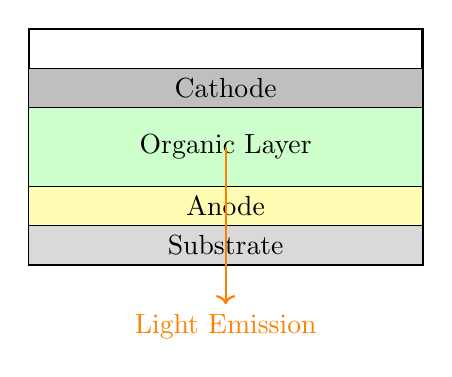
\begin{tikzpicture}
    % Layers
    \draw[thick] (0,0) rectangle (5,3);
    \draw[fill=gray!30] (0,0) rectangle (5,0.5) node[midway]{Substrate};
    \draw[fill=yellow!30] (0,0.5) rectangle (5,1) node[midway]{Anode};
    \draw[fill=green!20] (0,1) rectangle (5,2) node[midway]{Organic Layer};
    \draw[fill=gray!50] (0,2) rectangle (5,2.5) node[midway]{Cathode};
    
    \draw[->, orange, thick] (2.5, 1.5) -- (2.5, -0.5) node[below]{Light Emission};
\end{tikzpicture}
\end{center}

\begin{center}
\captionof{table}{Working and Applications of OLED}
\begin{tabular}{|l|l|}
\hline
\textbf{Aspect} & \textbf{Description} \\ \hline
Working & Electron-hole recombination in organic layer produces light \\ \hline
Efficiency & High efficiency, low power consumption \\ \hline
Viewing Angle & Excellent (nearly 180$^{\circ}$) \\ \hline
Applications & Smartphones, TVs, wearable devices, lighting \\ \hline
Advantages & Thin, flexible, better contrast, faster response \\ \hline
\end{tabular}
\end{center}
\end{solutionbox}
\begin{mnemonicbox}
``VIEWS technology'' (Vibrant colors, Incredible contrast, Excellent angle, Wide application, Self-emitting)
\end{mnemonicbox}

\orquestionmarks{4}{c}{7}
\textbf{Explain working of solar battery charger circuits.}

\begin{solutionbox}
\textbf{Answer}:
Solar battery charger converts solar energy to electrical energy to charge batteries.

\begin{center}
\begin{tikzpicture}[node distance=2.5cm, auto]
    \node [gtu block] (Solar) {Solar Panel};
    \node [gtu block, right of=Solar] (Control) {Charge\\Controller};
    \node [gtu block, right of=Control] (Reg) {Voltage\\Regulator};
    \node [gtu block, right of=Reg] (Bat) {Battery};
    \node [gtu block, below of=Reg] (Load) {Load};
    
    \draw [gtu arrow] (Solar) -- (Control);
    \draw [gtu arrow] (Control) -- (Reg);
    \draw [gtu arrow] (Reg) -- (Bat);
    \draw [gtu arrow] (Bat) |- (Load);
    
    \node [below of=Control, node distance=1.5cm] (Ind) {Indicator};
    \draw [gtu arrow] (Control) -- (Ind);
\end{tikzpicture}
\end{center}

\begin{center}
\captionof{table}{Components and Their Functions}
\begin{tabular}{|l|l|}
\hline
\textbf{Component} & \textbf{Function} \\ \hline
Solar Panel & Converts sunlight to DC electricity \\ \hline
Charge Controller & Prevents overcharging and deep discharge \\ \hline
Voltage Regulator & Stabilizes voltage to appropriate charging level \\ \hline
Battery & Stores electrical energy \\ \hline
Indicator Circuit & Shows charging status and battery level \\ \hline
\end{tabular}
\end{center}

\begin{itemize}
    \item \textbf{Working principle}: Photovoltaic effect converts sunlight to electricity
    \item \textbf{Regulation}: Prevents overcharging using voltage/current regulation
    \item \textbf{Protection}: Includes reverse current protection to prevent battery discharge at night
    \item \textbf{Types}: PWM (Pulse Width Modulation) and MPPT (Maximum Power Point Tracking)
\end{itemize}
\end{solutionbox}
\begin{mnemonicbox}
``SCORE system'' (Solar Conversion, Overcharge protection, Regulation, Energy storage)
\end{mnemonicbox}

\questionmarks{5}{a}{3}
\textbf{Draw a block diagram of regulated power supply.}

\begin{solutionbox}
\textbf{Answer}:
Regulated power supply provides stable DC output voltage despite variations in input or load.

\begin{center}
\begin{tikzpicture}[node distance=2.5cm, auto]
    \node [gtu block] (Trans) {Transformer};
    \node [gtu block, right of=Trans] (Rect) {Rectifier};
    \node [gtu block, right of=Rect] (Filt) {Filter};
    \node [gtu block, right of=Filt] (Reg) {Voltage\\Regulator};
    \node [gtu block, right of=Reg] (Out) {Output};
    
    \draw [gtu arrow] (Trans) -- (Rect);
    \draw [gtu arrow] (Rect) -- (Filt);
    \draw [gtu arrow] (Filt) -- (Reg);
    \draw [gtu arrow] (Reg) -- (Out);
\end{tikzpicture}
\end{center}
\end{solutionbox}
\begin{mnemonicbox}
``TRFO blocks'' (Transformer, Rectifier, Filter, Output regulator)
\end{mnemonicbox}

\questionmarks{5}{b}{4}
\textbf{Describe Transistor shunt Voltage Regulator.}

\begin{solutionbox}
\textbf{Answer}:
Transistor shunt regulator maintains constant output voltage by diverting excess current through a transistor in parallel with the load.

\begin{center}
\begin{circuitikz}
    \draw (0,0) to[V, l=$V_{in}$] (0,3) to[R, l=$R_S$] (3,3) -- (5,3) to[R, l=$R_L$] (5,0) -- (0,0);
    
    % Shunt transistor

    % Let's draw standard orientation
    \draw (3,1) node[npn] (Q) {};
    \draw (3,3) -- (Q.C);
    \draw (Q.E) -- (3,0) node[ground]{};
    
    % Zener reference
    \draw (1.5, 3) to[R] (1.5, 1) -- (Q.B);
    \draw (1.5, 1) to[zD, l=$D_Z$, invert] (1.5, 0) node[ground]{};
    
    \draw (5,3) to[short, -o] (6,3) node[right]{$V_{out}$};
    \draw (5,0) to[short, -o] (6,0);
\end{circuitikz}
\end{center}

\begin{center}
\captionof{table}{Transistor Shunt Regulator}
\begin{tabular}{|l|l|}
\hline
\textbf{Component} & \textbf{Function} \\ \hline
Zener & Provides reference voltage \\ \hline
Transistor & Shunts excess current \\ \hline
Series Resistor ($R_S$) & Drops excess voltage \\ \hline
Load Resistor ($R_L$) & Represents circuit being powered \\ \hline
\end{tabular}
\end{center}

\begin{itemize}
    \item \textbf{Working}: Transistor conducts more when output tries to increase
    \item \textbf{Advantage}: Simple circuit with good regulation
\end{itemize}
\end{solutionbox}
\begin{mnemonicbox}
``ZEST circuit'' (Zener reference, Excess current, Shunt transistor, Tension-free output)
\end{mnemonicbox}

\questionmarks{5}{c}{7}
\textbf{Draw and explain SMPS block diagram with its advantages and disadvantages.}

\begin{solutionbox}
\textbf{Answer}:
Switched Mode Power Supply (SMPS) uses switching regulation for high efficiency.

\begin{center}
\begin{tikzpicture}[node distance=2cm, auto]
    \node [gtu block] (AC) {AC Input};
    \node [gtu block, right of=AC] (EMI) {EMI\\Filter};
    \node [gtu block, right of=EMI] (Rect) {Rectifier\\\& Filter};
    \node [gtu block, right of=Rect] (Switch) {Switching\\Circuit};
    \node [gtu block, below of=Switch] (Feed) {Feedback};
    \node [gtu block, right of=Switch] (Trans) {Trans-\\former};
    \node [gtu block, right of=Trans] (OutRect) {Output\\Rect/Filter};
    \node [gtu block, right of=OutRect] (DC) {DC Output};
    
    \draw [gtu arrow] (AC) -- (EMI);
    \draw [gtu arrow] (EMI) -- (Rect);
    \draw [gtu arrow] (Rect) -- (Switch);
    \draw [gtu arrow] (Switch) -- (Trans);
    \draw [gtu arrow] (Trans) -- (OutRect);
    \draw [gtu arrow] (OutRect) -- (DC);
    \draw [gtu arrow] (DC) |- (Feed);
    \draw [gtu arrow] (Feed) -- (Switch);
\end{tikzpicture}
\end{center}

\begin{center}
\captionof{table}{Advantages and Disadvantages of SMPS}
\begin{tabular}{|l|l|}
\hline
\textbf{Advantages} & \textbf{Disadvantages} \\ \hline
High efficiency (80-95\%) & Complex circuit design \\ \hline
Small size and lightweight & Generates high-frequency noise \\ \hline
Wide input voltage range & EMI/RFI interference \\ \hline
Good regulation & Higher cost for low power \\ \hline
Lower heat generation & Difficult troubleshooting \\ \hline
\end{tabular}
\end{center}

\begin{itemize}
    \item \textbf{Working principle}: Rapidly switches power on/off at high frequency
    \item \textbf{Size reduction}: Higher switching frequency allows smaller transformers
    \item \textbf{Applications}: Computers, TVs, mobile chargers, LED drivers
\end{itemize}
\end{solutionbox}
\begin{mnemonicbox}
``SWEEP advantages'' (Small size, Widerange input, Efficient, Economical, Precise regulation)
\end{mnemonicbox}

\orquestionmarks{5}{a}{3}
\textbf{Draw voltage regulator using three terminal IC 7812.}

\begin{solutionbox}
\textbf{Answer}:
Three terminal IC 7812 provides fixed +12V regulated output voltage.

\begin{center}
\begin{circuitikz}
    \draw (0,0) node[left]{$V_{in}$} to[short, o-] (1,0) -- (1,1);
    \draw (1,1) rectangle (3,2.5);
    \node at (2, 1.75) {7812};
    \node at (1, 1.2) {\tiny IN};
    \node at (3, 1.2) {\tiny OUT};
    \node at (2, 1) {\tiny GND};
    
    \draw (3,1.2) -- (4,1.2) to[short, -o] (5,1.2) node[right]{$V_{out}$ (+12V)};
    \draw (2,1) -- (2,0) node[ground]{};
    \draw (1,1.2) -- (0.5, 1.2); % Input line
    
    \draw (1,1.2) to[C, l=$C_1$] (1,0) node[ground]{};
    \draw (4,1.2) to[C, l=$C_2$] (4,0) node[ground]{};
\end{circuitikz}
\end{center}

\begin{itemize}
    \item \textbf{Components}: 7812 regulator IC and filter capacitors
    \item \textbf{Pin configuration}: Input, Ground, Output
    \item \textbf{Features}: Internal current limiting and thermal shutdown
\end{itemize}
\end{solutionbox}
\begin{mnemonicbox}
``IGO pins'' (Input, Ground, Output)
\end{mnemonicbox}

\orquestionmarks{5}{b}{4}
\textbf{Describe Transistor series Voltage Regulator}

\begin{solutionbox}
\textbf{Answer}:
Transistor series regulator controls output voltage by varying the conductivity of a series transistor.

\begin{center}
\begin{circuitikz}
    \draw (0,0) to[V, l=$V_{in}$] (0,3) to[short] (1,3);

    % Let's draw standard horizontal npn
    \draw (2,3) node[npn] (Q) {};
    \draw (0,3) -- (Q.C);
    \draw (Q.E) -- (4,3) to[short, -o] (5,3) node[right]{$V_{out}$};
    \draw (5,3) to[R, l=$R_L$] (5,0) -- (0,0);
    \draw (5,0) to[short, -o] (6,0);
    
    % Zener Ref
    \draw (0,3) to[R, l=$R$] (0.5, 1.5) -- (Q.B);
    \draw (0.5, 1.5) to[zD, l=$D_Z$, invert] (0.5, 0) node[ground]{};
\end{circuitikz}
\end{center}

\begin{center}
\captionof{table}{Features of Series Voltage Regulator}
\begin{tabular}{|l|l|}
\hline
\textbf{Feature} & \textbf{Description} \\ \hline
Control Element & Transistor acts as variable resistor in series \\ \hline
Reference & Zener diode provides stable reference voltage \\ \hline
Regulation & Feedback adjusts transistor conductivity \\ \hline
Efficiency & Better than shunt regulator for high current loads \\ \hline
\end{tabular}
\end{center}

\begin{itemize}
    \item \textbf{Working principle}: Transistor conductivity changes to maintain constant output
    \item \textbf{Advantage}: More efficient than shunt regulators for higher currents
\end{itemize}
\end{solutionbox}
\begin{mnemonicbox}
``CERT circuit'' (Control transistor, Efficient design, Reference voltage, Transistor in series)
\end{mnemonicbox}

\orquestionmarks{5}{c}{7}
\textbf{Draw and explain UPS block diagram with its advantages and disadvantages.}

\begin{solutionbox}
\textbf{Answer}:
Uninterruptible Power Supply (UPS) provides emergency power when main supply fails.

\begin{center}
\begin{tikzpicture}[node distance=2.5cm, auto]
    \node [gtu block] (AC) {AC Input};
    \node [gtu block, right of=AC] (Surge) {Surge\\Protector};
    \node [gtu block, right of=Surge] (Rect) {Rectifier/\\Charger};
    \node [gtu block, right of=Rect] (Inv) {Inverter};
    \node [gtu block, right of=Inv] (Filt) {Output\\Filter};
    \node [gtu block, right of=Filt] (Out) {AC Output};
    
    \node [gtu block, below of=Rect] (Bat) {Battery};
    
    \draw [gtu arrow] (AC) -- (Surge);
    \draw [gtu arrow] (Surge) -- (Rect);
    \draw [gtu arrow] (Rect) -- (Inv);
    \draw [gtu arrow] (Inv) -- (Filt);
    \draw [gtu arrow] (Filt) -- (Out);
    
    \draw [gtu arrow] (Rect) -- (Bat);
    \draw [gtu arrow] (Bat) -| (Inv);
    
    % Control can be implied or drawn
    \node [below of=Inv, node distance=1.5cm] (Control) {Control Circuit};
    \draw [gtu arrow, dashed] (Control) -- (Rect);
    \draw [gtu arrow, dashed] (Control) -- (Inv);
\end{tikzpicture}
\end{center}

\begin{center}
\captionof{table}{Advantages and Disadvantages of UPS}
\begin{tabular}{|l|l|}
\hline
\textbf{Advantages} & \textbf{Disadvantages} \\ \hline
Provides backup power & Limited backup time \\ \hline
Protects from voltage fluctuations & Regular battery maintenance \\ \hline
Surge protection & Initial high cost \\ \hline
Smooth power transition & Noise during operation \\ \hline
Power conditioning & Lower efficiency in standby \\ \hline
\end{tabular}
\end{center}

\begin{itemize}
    \item \textbf{Types}: Offline/Standby, Line-interactive, Online/Double-conversion
    \item \textbf{Applications}: Computers, medical equipment, data centers, telecommunications
    \item \textbf{Working}: Normally passes main power while charging battery; switches to battery power during outage
\end{itemize}
\end{solutionbox}
\begin{mnemonicbox}
``POWER backup'' (Protection from Outages, Waveform conditioning, Emission-free, Reliability boost)
\end{mnemonicbox}

\end{document}
